\subsection{Основные функции и обобщенные функции, сходимость в пространстве основных функций. Регулярная обобщённая функция. Носитель обобщённой функции}
%aut: Slava
%ref: Владимиров, стр. 65
\subsubsection{Основа}
\textsc{Пример мотивации.} Найти плотность материальной точки. Интеграл
плотности по
области, содержащей эту точку должен давать её массу.

Рассмотрим однородный шар $ U_\delta $ в пространстве\footnote{Для удобства
вектор $ \mathbf x $ будет записываться как просто $ x $.} $ \mathbb R^3 $ массы $ m = 1 $ в начале координат. Плотность этого шара выражается
соотношениями\footnote{См. формулу объёма шара.}  
\[
  f_\delta(x) = \begin{cases}
    0, & |x| > \delta,\\
    \dfrac{3}{4\pi \delta^3}, & |x| < \delta.
  \end{cases}
\]
Теперь нужно устремить его радиус $ \delta \to 0 $. Классический предел не
даёт вменяемого результата, поэтому рассмотрим \emph{слабый предел}. Именно, для
каждой непрерывной функции $ \varphi $ найдём предел 
\[
  \lim_{\delta \to 0} \int f_\delta(x)\varphi(x) \, dx = \varphi(0).
\]
Действительно, для любого $ \varepsilon > 0 $ имеем такую $ \delta_0 $, что при
всех $ \delta < \delta_0 $ 
\begin{multline*}
    \left| \int f_\delta(x)\varphi(x)\, dx - \varphi(0) \right| =
    \frac{3}{4\pi\delta^3} \left| \int_{|x| < \delta} \varphi(x) - \varphi(0)\,dx
    \right| \leqslant\\\leqslant
    \frac{3}{4\pi\delta^3} \int_{|x|<\delta}|\varphi(x)-\varphi(0)|\, dx <
    \varepsilon \frac{3}{4\pi\delta^3} \int_{|x| <\delta} dx = \varepsilon.
\end{multline*}
Здесь была использована непрерывность $ \varphi $, а также общие свойства
интегралов.

\sloppy
Назовём тогда \emph{$ \delta $-функцией Дирака} полученный
функционал\footnote{<<Настоящий>> аргумент $ \delta $ --- функция. Запись $
\delta(x) $ удобна и обоснована. Применение функционала к функции будем записывать как ($\delta,
\varphi  $).} $ \delta(x)\colon C(\mathbb R^3) \to \mathbb R $, $(\delta, \varphi) = \lim\int
f_\delta\varphi\,dx = \varphi(0)$. Для точки массой $ m $, находящейся в
$ x_0  $, имеем плотность $
m\delta(x - x_0) $. Чтобы получить её массу, подействуем нашей функцией $ (m\delta, 1)
= m\cdot1(x_0) = m$ на $ \varphi\equiv 1 $. Полученный функционал линеен и
непрерывен\footnote{Определение непрерывности см. далее.}. 

\subsubsection{Пространство основных функций $ \mathcal D $} Функция $ \varphi $ в
нашем примере, как говорят, является \emph{основной функцией} для $ \delta(x) $.
Она достаточно хороша, чтобы соответствующий предел существовал. Ясно, что чем
<<лучше>> пространство основных функций, тем больше существует линейных непрерывных
функционалов на нем. 

Пространство основных функций $ \mathcal D = \mathcal D(\mathbb R^n) $ ---
все финитные\footnote{Носитель --- замыкание множества, на котором функция
отлична от нуля (обозн. $ \operatorname{supp} $) --- компактен (ограничен).} бесконечно дифференцируемые в $
\mathbb R^n $ функции вместе с введённым понятием сходимости.

\paragraph{Сходимость в $ \mathcal D $.} Скажем, что последовательность функций $ \varphi_k \in
\mathcal D$ сходится к функции $ \varphi \in \mathcal D $, если 
\begin{enumerate}
  \item Существует такое число $ R > 0 $, что $ \operatorname{supp} \varphi_k \subset U_R $.
  \item Для любого мультииндекса $ \alpha = (\alpha_1, \alpha_2, \ldots,
    \alpha_n) $ выполняется\footnote{Обозначения: $\alpha_k = 0, 1, \ldots$;
    $|\alpha| := \sum \alpha_k$; $\partial^\alpha f(x) :=
  \frac{\partial^{|\alpha|}f(x_1, \ldots, x_n)}{\partial x_1^{\alpha_1}
\ldots\partial_n^{\alpha_n}}$. Знаком $ \rightrightarrows $ обозначается
равномерная сходимость: $ \exists \delta \forall\varepsilon\colon |x-x_0| < \delta
\Rightarrow |f(x) - f(x_0)| < \varepsilon $.} 
  \[
      \partial^\alpha \varphi_k(x) \rightrightarrows \partial^\alpha\varphi(x),
      \quad k \to \infty.
  \]
\end{enumerate}

\paragraph{Примеры непрерывных операторов из $ \mathcal D $ в $ \mathcal D $.} 
\begin{enumerate}
  \item Докажем по определению\footnote{Определение: $ f_k \to f
      \Rightarrow Lf_k \to Lf $, что равносильно ($ g_k = |f - f_k| $) $ g_k \to 0
    \Rightarrow Lg_k \to 0 $.} непрерывность оператора дифференцирования, то есть
    что $ \varphi_k \to 0 $ влечёт $
    \partial^\alpha\varphi_k \to 0 $. Первое требование выполняется очевидным
    образом. Второе требование следует из соотношения $ \partial^\beta \circ
    \partial^\alpha = \partial^{\alpha + \beta} $.
  \item Аналогично показывается, что непрерывен оператор $ (l, \varphi(x)) :=
    \varphi(Ax + B) $, $ A \neq 0 $.
  \item  Непрерывна операция умножения на функцию\footnote{$C^\infty(\mathbb
      R^n)$ есть
    пространство бесконечно дифференцируемых на $ \mathbb R^n $ функций.} $
  a(x)\in C^\infty(\mathbb R^n) $.
\end{enumerate}
Заметим, что все перечисленные операции переводят функции из $ \mathcal D $ в
функции из $ \mathcal D $ (это обособленные факты).

\paragraph{Примеры ненулевых функций из $ \mathcal D $.}
\emph{<<Шапочка>>}: 
\[
  \omega_\varepsilon(x) = \begin{cases}
    C_\varepsilon\exp \left[ - \frac{\varepsilon^2}{\varepsilon^2 - |x|^2}
    \right], & |x| < \varepsilon,\\
    0, & |x| \geqslant \varepsilon.
  \end{cases}
\]
В дальнейшем она будет играть роль функции усреднения, поэтому $ C_\varepsilon $
выбираем так, чтобы $ \int \omega_\varepsilon(x)\,dx=1 $. Легко
заметить\footnote{Путём подстановки $ \xi = x/\varepsilon $ ($ x \in \mathbb R^n
  $) и деления числителя
и знаменателя на $ \varepsilon^2 $.}, что 
\[
    \omega_\varepsilon(x) = \frac{1}{\varepsilon^n}\omega_1 \left(
    \frac{x}{\varepsilon} \right).
\]

\begin{wrapfigure}{l}{0.4\textwidth}
  \centering
  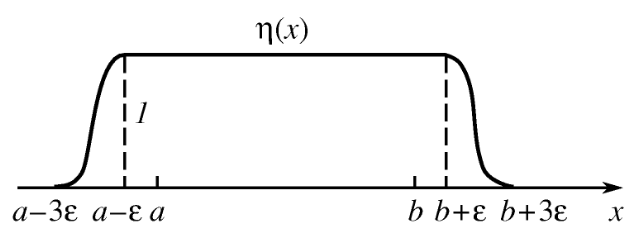
\includegraphics[width=0.4\textwidth]{img/eta(x).png}
\end{wrapfigure}
Найдём ещё целый класс функций из $ \mathcal D $.
% \begin{figure}[H]
%   \centering
%   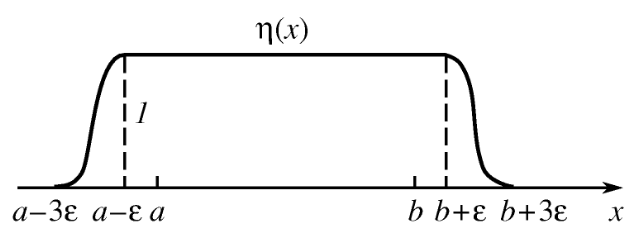
\includegraphics[width=0.3\textwidth]{img/eta(x).png}
% \end{figure}
Именно, для \textsl{произвольной области} $ G $ и произвольного $ \varepsilon $
докажем, что функция\footnote{В области $ G_{2\varepsilon} $ каждая точка
области $ G $ гомотетична продолжена на $ 2\varepsilon $. По поводу бесконечной
дифференцируемости см.
\emph{Формулу Лейбница} (производной интеграла с параметром). Интеграл равен единице благодаря чётности шапочки.} 
\begin{gather*}
  \eta(x) = \int_{G_{2\varepsilon}} \omega_\varepsilon(x-y)\, dy \in
  C^\infty(\mathbb R^n),\\
  0 \leqslant \eta(x) \leqslant \int\omega_\varepsilon(x-y)\, dy = 1
\end{gather*}
принадлежит $ \mathcal D $. Пусть $ \Omega = U(\varepsilon) \cap
G_{2\varepsilon}$.  Понятно, что  
\[
  \eta(x) = \int_{\Omega} \omega_\varepsilon(x - y)\, dy = \begin{cases}
    1, & x \in G_\varepsilon,\\
    0, & x\notin G_{3\varepsilon}.
  \end{cases}
\]

\subsubsection{Пространство обобщённых функций $ \mathcal D' $}
\emph{Обобщённой функцией} называют линейный непрерывный\footnote{В реальности
  не найдено ни одного линейного непрерывного функционала. Их существование
гарантируется лишь аксиомой выбора.} функционал на $
\mathcal D $. 

Множество таких функций $ \mathcal D' $ линейное\footnote{С введёнными
  операциями сложения и умножения на число: $ (\lambda f + \mu g,\varphi) =
\lambda(f,\varphi) + \mu(g,\varphi) $. Здесь функционал $ \lambda f + \mu g $,
как легко убедиться, принадлежит $ \mathcal D' $.}.

\paragraph{Сходимость в $ \mathcal D' $.}
Скажем, что последовательность $ f_k \in \mathcal D' $ сходится к $ f \in
\mathcal D' $, если для любой $ \varphi \in \mathcal D $ последовательность $
(f_k, \varphi) \in \mathbb R$ сходится к $ (f, \varphi) \in \mathbb R $.

Множество линейный непрерывных функционалов вместе с введённым понятием
сходимости называют \emph{пространством $ \mathcal D' $}. Важным свойством $
\mathcal D' $ является его полнота\footnote{То есть гарантия сходимости
фундаментальной последовательности --- всегда $ \lim(f_k, \varphi) \in \mathcal
D'$.}.

\paragraph{Носитель обобщённой функции.} Говорят, что обобщённая функция $ f $
\emph{равна нулю в области\footnote{В точках значение функционала не
    определяется.
Далее будем использовать обозначение $ f = x $, $ x\in G $.} $ G $}, если $ (f,\varphi)  = 0 $ для
всех $ \varphi
\in \mathcal D(G)$\footnote{Говорят, что $ \varphi \in\mathcal D(G) $, если $ \varphi \in \mathcal
D$ и $ \operatorname{supp} \varphi \in G $.}. В частности, $ f, g \in \mathcal
D' $ называют равными, если $ (f,\varphi) = (g,\varphi) $ для всех $ \varphi \in
\mathcal D(\mathbb R^n)$. Понятно, что если $ \tilde G \subset G $, то $ f $
обращается в нуль и на $ \tilde G $. Оказывается, верно и обратное.

\begin{theorem} Если обобщённая функция $ f $ равна нулю в (некоторой данной) окрестности любой
  точки области $ G $, то она равна нулю и во всей области $ G $.
\end{theorem}
\begin{proof}
Фиксируем произвольную функцию $ \varphi \in \mathcal D(G) $. Её носитель
компактен. Покроем его бесконечной открытой системой множеств, на которых $ f =
0$ и выделим из неё конечную подсистему\footnote{См. \emph{лемма Гейне --
Борелля}.} Не теряя общности, будем считать, что полученная система есть система
шаров $ U(x_k; r_k) $. Понятно\footnote{Строгое обоснование этого шага: возьмём
у каждой точки, окрестность, которая с замыканием лежит в элементах покрытия.
Снова выделим конечное подпокрытие. Объединим все элементы нового покрытия,
которые принадлежат некоторому элементу старого.}, что всегда можно немного уменьшить радиус $ r_k
$ до $ r'_k < r_k $ у этих шаров так, чтобы они по-прежнему покрывали $ \operatorname{supp}\varphi
$. Как было выяснено выше, существуют основные функции $ h_k(x) $ со
свойствами 
\[
  h_k(1) = 1, \quad x \in U(x_k; r'_k), \quad \operatorname{supp}h_k \subset
  U(x_k; r_k).
\]
Положим  
\[
  h(x) := \sum_{k=1}^N h_k(x), \quad \varphi_k(x) := \varphi(x)
  \frac{h_k(x)}{h(x)}.
\]
Теперь поскольку $ \varphi_k \in \mathcal D(U(x_k; r_k)) $, 
\[
  (f,\varphi) = \left(f, \sum_{k=1}^N \varphi_k\right) =
  \sum_{k=1}^N(f,\varphi_k) = 0.
\]
\end{proof}

\emph{Нулевым множеством} $ \mathcal O_f $ функции $ f $ теперь назовём объединение всех окрестностей, где $ f
= 0$; а её \emph{носителем} --- дополнение $ \operatorname{supp} f = \mathbb R^n
\setminus\mathcal O_f$. Если последнее множество ограничено, то $ f $ называют
\emph{финитной}. Таким образом, $ f = 0 $ в любой области вне $ \operatorname{supp} f $
и $ f\neq 0 $ для окрестности любой точки из $ \operatorname{supp}f $.

Сужение, или \emph{локальный элемент}, обобщённой функции $ f $ на $ G $  
\[
  (f_G, \varphi) = (f, \varphi), \quad \varphi \in\mathcal D(G),
\]
как легко проверить, само линейно и непрерывно. Справедлива также обратная
\begin{theorem}[о кусочном склеивании]
  Пусть система областей $ G_\alpha $ покрывает $ \mathbb R^n $ и заданы $
  f_\alpha $ на $ \mathcal D(G_\alpha) $, причём $ f_\alpha = f_\beta $, $ x \in
  G_\alpha \cap G_\beta$. Тогда существует единственная обобщённая функция $ f
  \in\mathcal D' $, имеющая $ f_\alpha $ своими локальными элементы на $
  G_\alpha $ при всех $ \alpha $.
\end{theorem}

\subsubsection{Регулярные обобщённые функции}
Простейший пример обобщённой функции порождает локально
интегрируемая\footnote{То есть функция, интегрируемая на
любом компактном подмножестве.} в $ \mathbb R^n
$ функция $ f(x) $: 
\[
  (f,\varphi) := \int f(x)\varphi(x)\,dx, \quad \varphi \in \mathcal D.
\]
Из линейности интеграла и теоремы о предельном переходе под его знаком следует
справедливость данного определения.

Такие обобщённые функции называют \emph{регулярными}, все остальные назовают
\emph{сингулярными}.

\begin{theorem}[Дюбуа -- Реймон]
  Для того чтобы локально интегрируемая в $ G $ функция $ f(x) $ обращалась в
  нуль в области $ G $ в смысле обобщённых функций, необходимо и достаточно,
  чтобы $ f(x) = 0 $ в $ G $.
\end{theorem}
\begin{proof} Достаточность очевидна. Необходимость следует из \emph{основного
  вариационного принципа}.
\end{proof}
Эта лемма позволяет построить взаимно однозначное соответствие между функцией $
f(x)$ и обобщённой функцией\footnote{Тут следует считать эквивалентными функции
$ f_1(x) $, $ f_2(x) $, если они отличаются на множестве меры нуль.} $ (f, \varphi) $. При этом носитель $ f(x) $
совпадает с носителем $ f $.

Из той же теоремы о предельном переходе под знаком интеграла следует, что если
последовательность $ f_k(x) \rightrightarrows f(x)$ на каждом компакте, то $ f_k \to f \in
\mathcal D'(\mathbb R^n) $.

Будем говорить, что $ f \in C^p(G) $, если $ f_G(x) \in C^p(G) $.
